% !TeX root = ../main.tex
\chapter{Project 01: Secure State Estimation}

\section{Objectives}
The aim of this task is the secure state estimation of a static system, $A = I$ by implementing IJAM and ISTA algorithms. Furthere, it is required to enhance the performance of the algorithms by tuning hyper parameters.

\section{Setting of the problem}
We are considering the following static, autonomous LTI system under adversarial attack on the sensors, where $A = I$, meaning that the states does not change overtime. It is further assumed that the value of the attack remains constant.

\begin{equation}
    \begin{cases}
        \tilde {x}(k+1) = A\tilde{x}(k) \\
        y(k) = C\tilde{x}(k) + \tilde{a} + \eta
    \end{cases}
\end{equation}

where $\tilde{a}$ is the real attack vector and the measurement vector $y$ tampered by attack and the measurements are corrupted with the nosie vector $\eta$ a normal distribution with standard deviation $\sigma = 10^{-2}$.

The dimension of the vectors is as follows:
\begin{itemize}
	\item the number of the states $n = 15$
	\item the number of the sensors, length of the measurement sensor $q = 30$
	\item the number of the attacks $h = 2$
\end{itemize}

In this exercise, $C$ is initialized with a standard normal distribution $\mathcal{N}(0,1)$, the components of the attack vector $\tilde{a}_i$ can assume random values uniformly distributed in the range $\left[-5, 4\right] \cup \left[4,5 \right]$, and finally the state components are initialized with random values uniformly distributed in the range $\left[-3, 2\right] \cup \left[2,3 \right]$.


Step criterion recommende for IJAM and ISTA is as follows:
\[
T_{\max} = \| x(T_{\max}+1) - x(T_{\max}) \|_2^2 < \delta, \quad \text{where} \quad \delta = 10^{-10}
\]

Not knowing the position of the attacks, the problem grows in a combinatorial manner. Hence, a partial lasso problem is considered for solving this problem. The optimization problem to be solved in order to estimate both the state as well as the attack is as follows:
\begin{equation}
    \min\limits_{x \in \mathbb{R}^n, \: a \in \mathbb{R}^q} \mathcal{F}(x,a) + \mathcal{G}(a)
\end{equation}
where 
\[
\mathcal{F}(x,a) = \frac{1}{2} \|Cx + a - y\|_2^2  \:\:\:\:\: \text{and} \mathcal{G}(a) = \lambda \|a\|_1 \:\:\:\:\ \text{with} \:\:\:\:\lambda >0
\]

However, since the problem is non-differentiable, the answer cannot be found analytically, and some iterative algorithms are used in order to solve this problem.


\section{Performing Secure State Estimation}
In this part 4 algorithm is used for solving the problem of secure state estimation - of which two are introduced in the course and the other two are invented as a modification of those two algorithms. The algorithms in the course are \textit{Inertial Jacobi Alternating minimization} (IJAM) and \textit{Iterative Soft Thresholding Algorithm} (ISTA). The other two algorithms in this report are called ``my IJAM'' and ``my ISTA'', the details of which are discussed in their relevant subsection.

\subsection{Inertial Jacobi Alternating minimization, or IJAM}
This is an iterative algorithm in order to solve the problem of secure state estimation. The idea here is to fix $a$, and solve the problem for $x$, which becomes a least-square problem, and then, the obtained $x$ is considered to be fixed and the optimization problem is solved for $a$, where the probelm becomes \textit{Proximal mapping of soft thresholding}, in order to enhance the numerical stability of the algorithm, an inertial term is added to the soft thresholding with the weight, $\nu$ with a value between 0 and 1; pay attention that if $\nu$ is set to one, we simply have soft thresholding without any inertia. Therefore, considering zero initial value for our vectors and a value of  the algorithm to solve the problem becomes as follows:
\begin{equation}
	\begin{cases}
		x(k+1) = C^{+}(y - a(k)) \\
		a(k+1) = \mathbb{S}_{\lambda \nu}\left[a(k) - \nu(Cx(k)+ a(k) - y)\right]
	\end{cases}
\end{equation}

It has been demonstrated that IJAM converge to the minimum of the partial Lasso we are aiming to solve. 


\subsection{Iterative Soft Thresholding Algorithm, or ISTA}
The approach adopted here is similar to the one adopted in IJAM, with the difference that when $a$ is considered to be constant, instead of solving the least-square problem using the analytical solution, a gradient decent algorithm is adopted and $x$ is decented toward the gradient of $\mathcal{F}$ for one step, $\tau = \nu$. Considering zero initial condition:

\begin{equation}
	\begin{cases}
		x(k+1) = x(k)- \nu C^{T}(Cx(k) + a(k) - y) \\
		a(k+1) = \mathbb{S}_{\lambda \nu}\left[a(k) - \nu(Cx(k)+ a(k) - y)\right]
	\end{cases}
\end{equation}

By iteration, also this problem converges to the minimum of the original problem mentioned in the setup section.

\subsection{My IJAM and MY ISTA}
In the first place, since the position of the attacks was not known, a partial lasso problem was defined to solve the problem. The idea here is to use IJAM and ISTA just in order to detect the position of the attacks. Knowing the position of the attacks, a normal algabric solution is adopted for solving the set of linear equations. Hence, after the IJAM and ISTA have estimated the position of the attacks, a diagonal support matrix,$M_a$, is shaped for a vector which have 1 only in the place of the corresponding attack. Then, the following problem is solving;
\begin{equation}
    \begin{bmatrix}
        \hat{x} \\
        \hat{a}
    \end{bmatrix} = 
    \left( C M_a \right)^{+} y
\end{equation}


\section{Analysis}
\subsection{Recovery Performance Matrices}
Two main recovery performance matrices are used in order to evaluate the performance of the algorithms:
\begin{itemize}
	\item mean of relative state estimation error $\frac{\|x(k) - \tilde{x}\|_2}{\|\tilde{x}\|_2}$
	\item mean of support attack error $\sum_j |1(\tilde{a}_j \neq 0) - 1(\hat{a}_j \neq 0)|$
\end{itemize}
Each algorithm is run for 20 times each time then the means are calculated.

Having used the hyperparameters recommended in the assignment which are:
\begin{itemize}
	\item $\lambda = 0.1$
	\item For ISTA $\nu = \frac{0.99}{\|G\|_2^2}$
	\item For IJAM $\nu = 0.7$
	\item $\delta = 10^{-10}$
\end{itemize}

It can be seen that both IJAM and ISTA result in almost the same recovery performance matrics. What can be observed from the graph bellow is that, despide having oscillatory behavior during the transient period, IJAM algorithm converges in almost one order of magnitude less number of iterations compared to ISTA algorithm. ISTA have a more stable behavior thanks to the fact that, while calculating $x$, it move one step in the reverse direction of the gradient, whereas in IJAM it solves a least square problem everytime. Given the fact that the same $delta$ is used for also ``my IJAM'' and ``my ISTA'', after reaching the convergence another step needs to be done which is doing the estimation using least-square solution of the probelm knowing the possition of the attacks.

The advantages of ``my IJAM'' and ``my ISTA'' is that it is about 80 to 90\% more precise compared to standard IJAM and ISTA, due to the fact that the least-square problem leads to the global optimal solution of the problem. Further, a lower value of $\delta$ can be set for IJAM and ISTA, since IJAM and ISTA are used only in order to detect the position of the attacks.

\begin{figure}[H] % h means "here", can also use t (top), b (bottom), p (page)
    \centering
    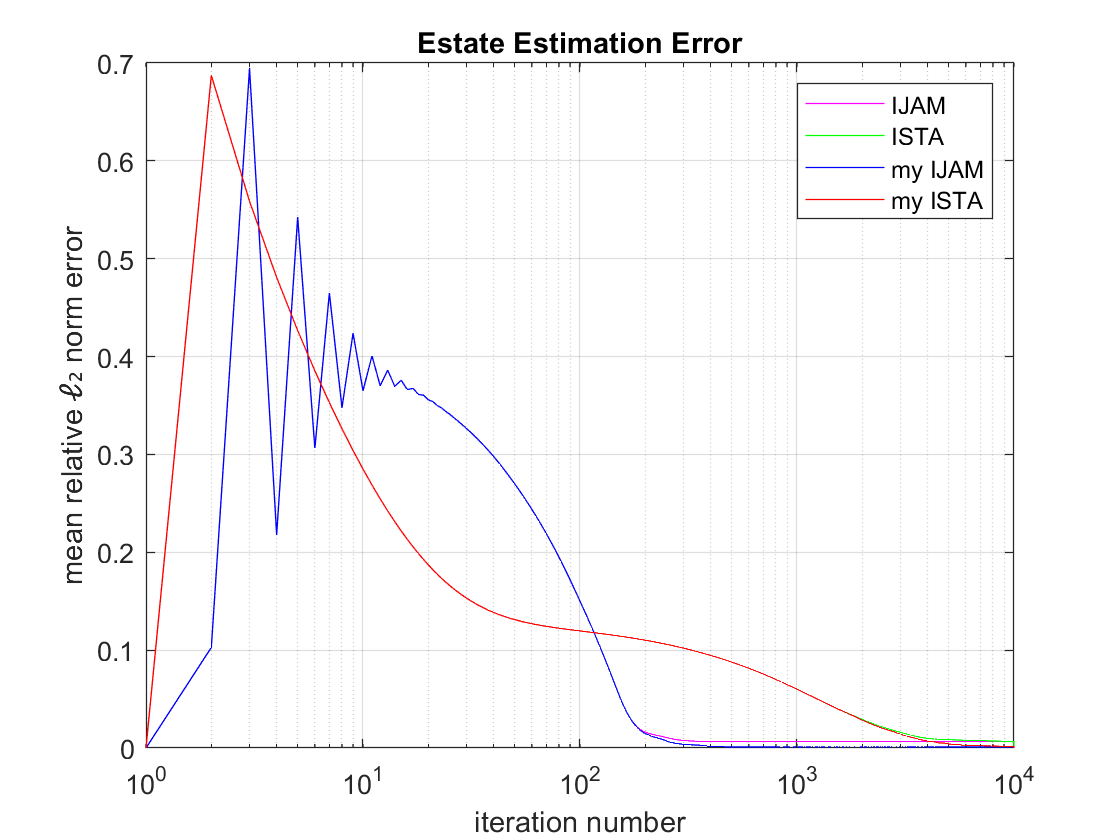
\includegraphics[width=0.75\textwidth]{mean_state_error.png} % Adjust width as needed
    \caption{Relative state error of the algorithms mention in the legend averaged in 20 run}
    \label{fig:example}
\end{figure}

\begin{figure}[H] % h means "here", can also use t (top), b (bottom), p (page)
    \centering
    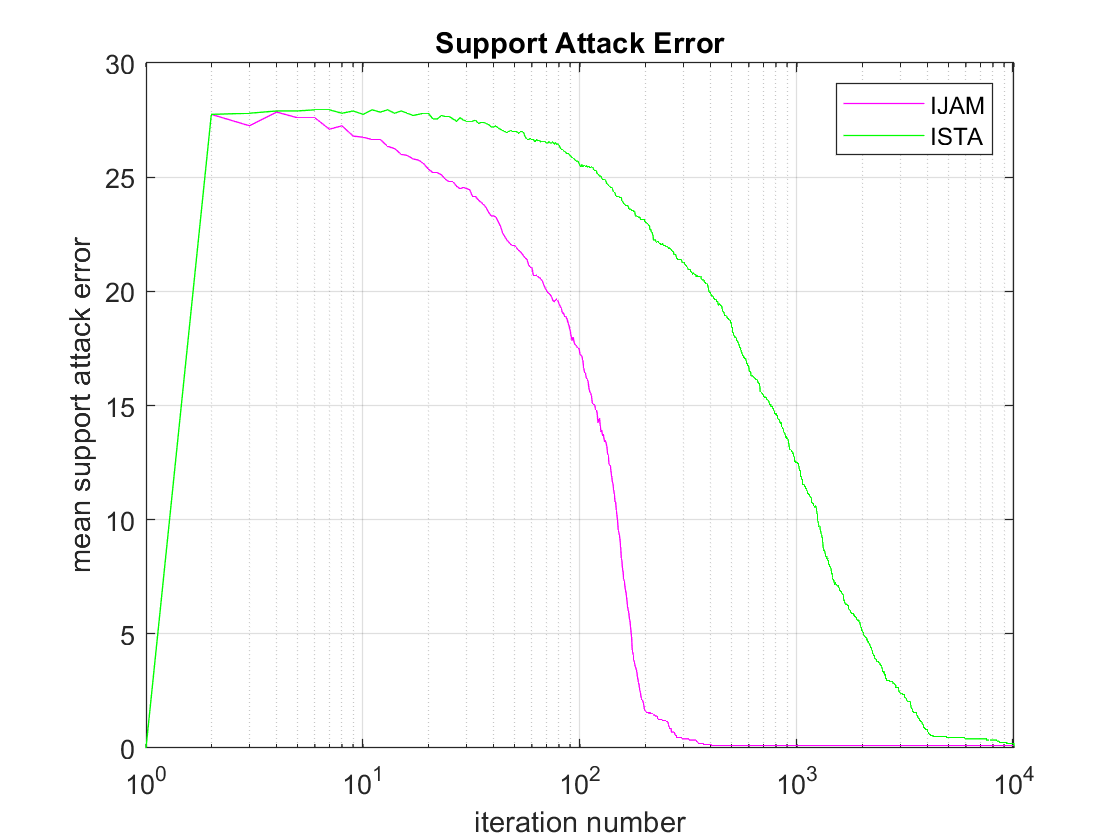
\includegraphics[width=0.75\textwidth]{mean_support_error.png} % Adjust width as needed
    \caption{Relative attack support error of the algorithms mention in the legend averaged in 20 run; my IJAM and my ISTA have the same performance as IJAM and ISTA, respectively.}
    \label{fig:example}
\end{figure}

\begin{figure}[H] % h means "here", can also use t (top), b (bottom), p (page)
    \centering
    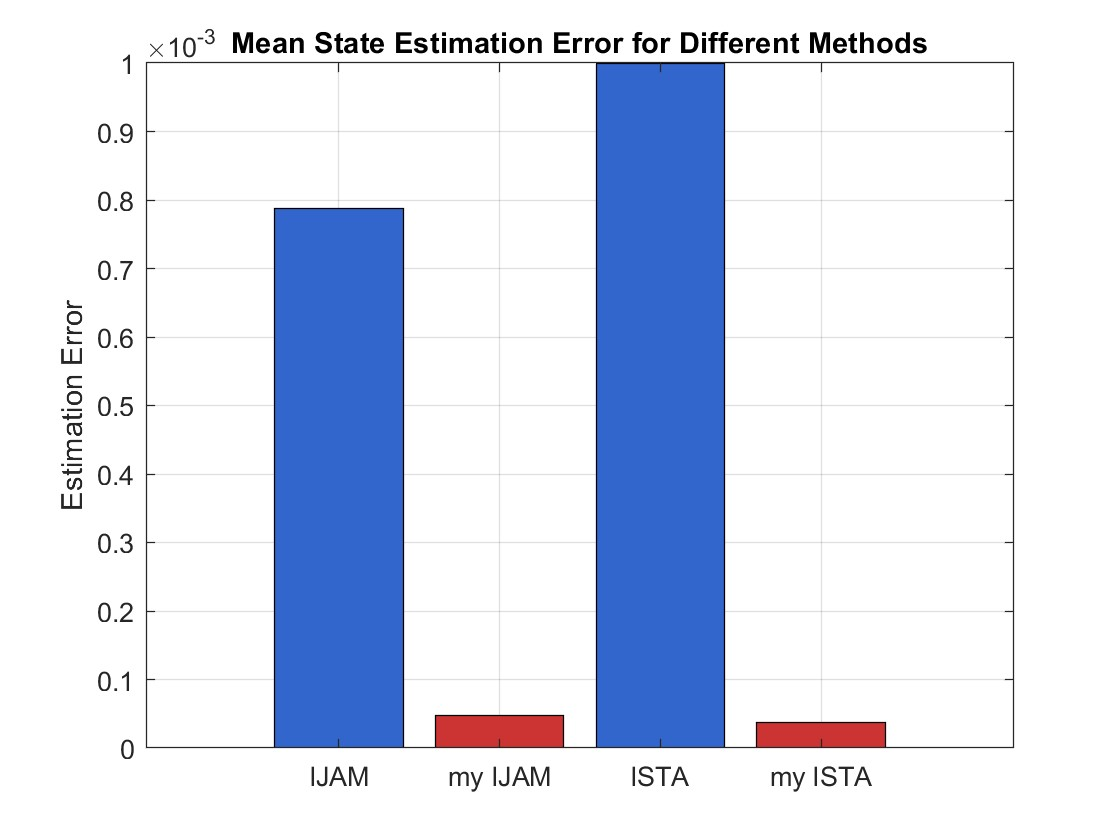
\includegraphics[width=0.65\textwidth]{precision_comparison.jpg} % Adjust width as needed
    \caption{comparison of the mean state error of the algorithms}
    \label{fig:example}
\end{figure}

Advantage of my ISTA, my IJAM, less average iteration, we don't need to estimate x to an exact precision, it is enough to find the position of the attacks, $90\%$ higher precision, since the problem is solved algabraically, we reach the global solution

\subsection{Tunning hyperparameters}
\subsubsection{changing $\lambda$}
$\lambda$ influence the weight of the first norm term in the partial lasso, which imposes sparcification. With large values of  $\lambda$, up to a certain extent, the convergence occurese in a less number of iterations, owing to the fact the soft-threshold pushed the values of attack vector to zero by a larger value. However, caution should be taken tuning lambda, since the larger value of $\lambda$ leads to over sparcification, which means underestimating small values of attack. This can be observed in the figures bellow where despide the fact that convergence occures in a less number of iterations for $lambda = 5$, but the algorithms cannot detect the position of the attack. On the other hand, if one sets the value of $lambda$ too small, other than leading to larger number of iterations, the algorithm considers noises and numberical inaccuracies as attack. 

\begin{figure}[H] % h means "here", can also use t (top), b (bottom), p (page)
    \centering
    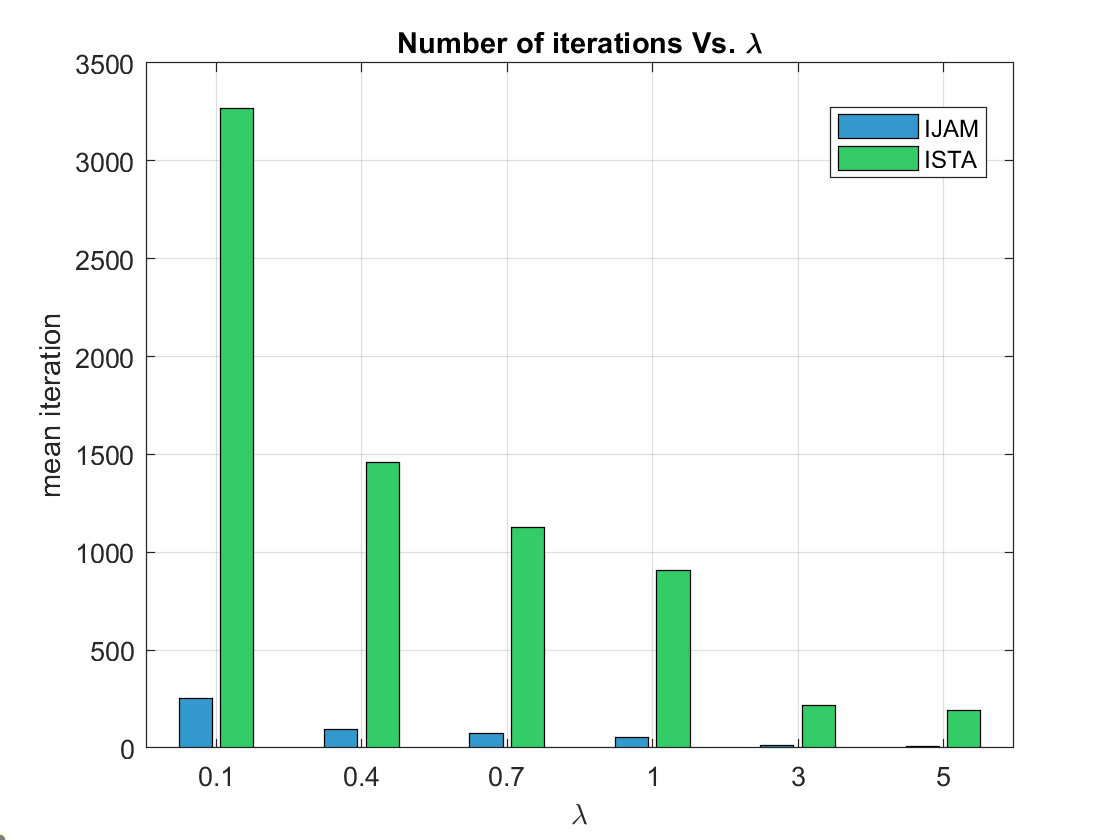
\includegraphics[width=0.65\textwidth]{iteration_vs_lambda.png} % Adjust width as needed
    \caption{Mean iteration required for convergance for different values of lambda}
    \label{fig:example}
\end{figure}

\begin{figure}[H] % h means "here", can also use t (top), b (bottom), p (page)
    \centering
    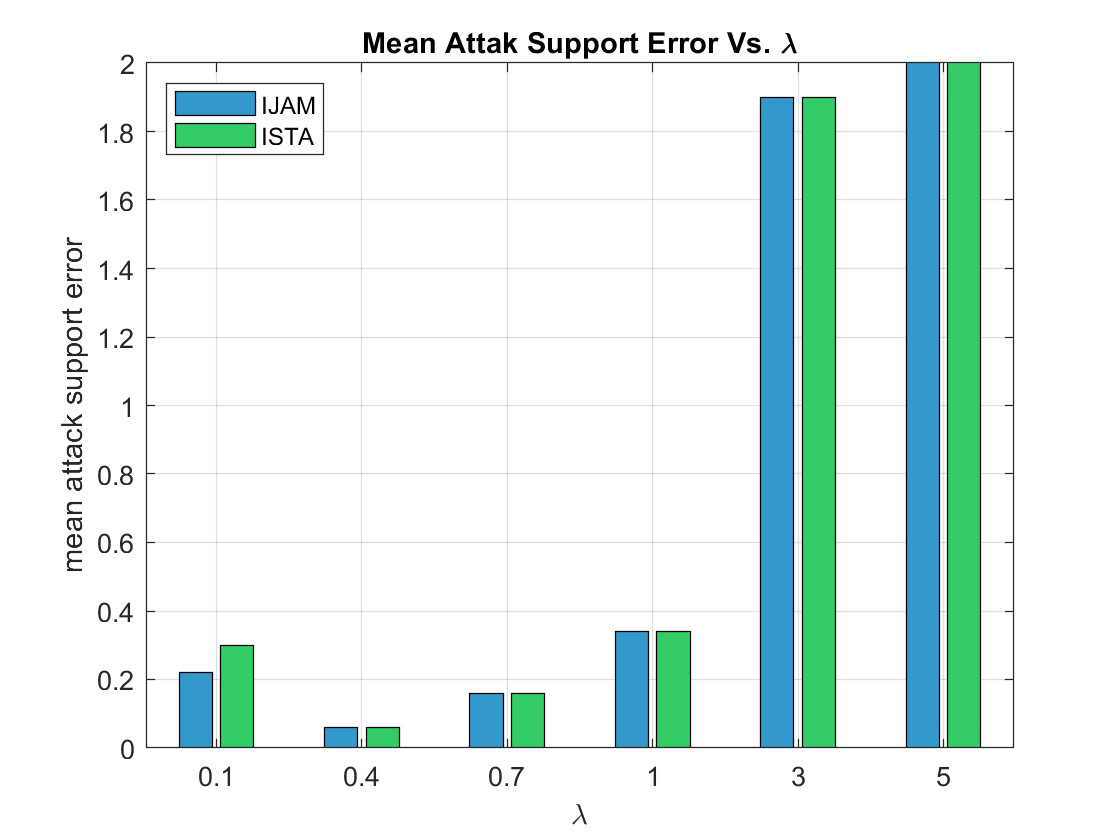
\includegraphics[width=0.65\textwidth]{attack_support_vs_lambda.png} % Adjust width as needed
    \caption{Mean attack support error of different methods for different values of lambda.}
    \label{fig:example}
\end{figure}


\subsubsection{changing $\nu$}
For the value of $\nu = 1$, we get the original algorithm for solving the problem; that is, no intertia is introduced in order to enhance the numerical stability of soft-thresholding operator, which is the case considering the state to be constant. However, for the range of  0 to 1, an inertia is introduced in the soft-thresholding. 

\begin{figure}[H] % h means "here", can also use t (top), b (bottom), p (page)
    \centering
    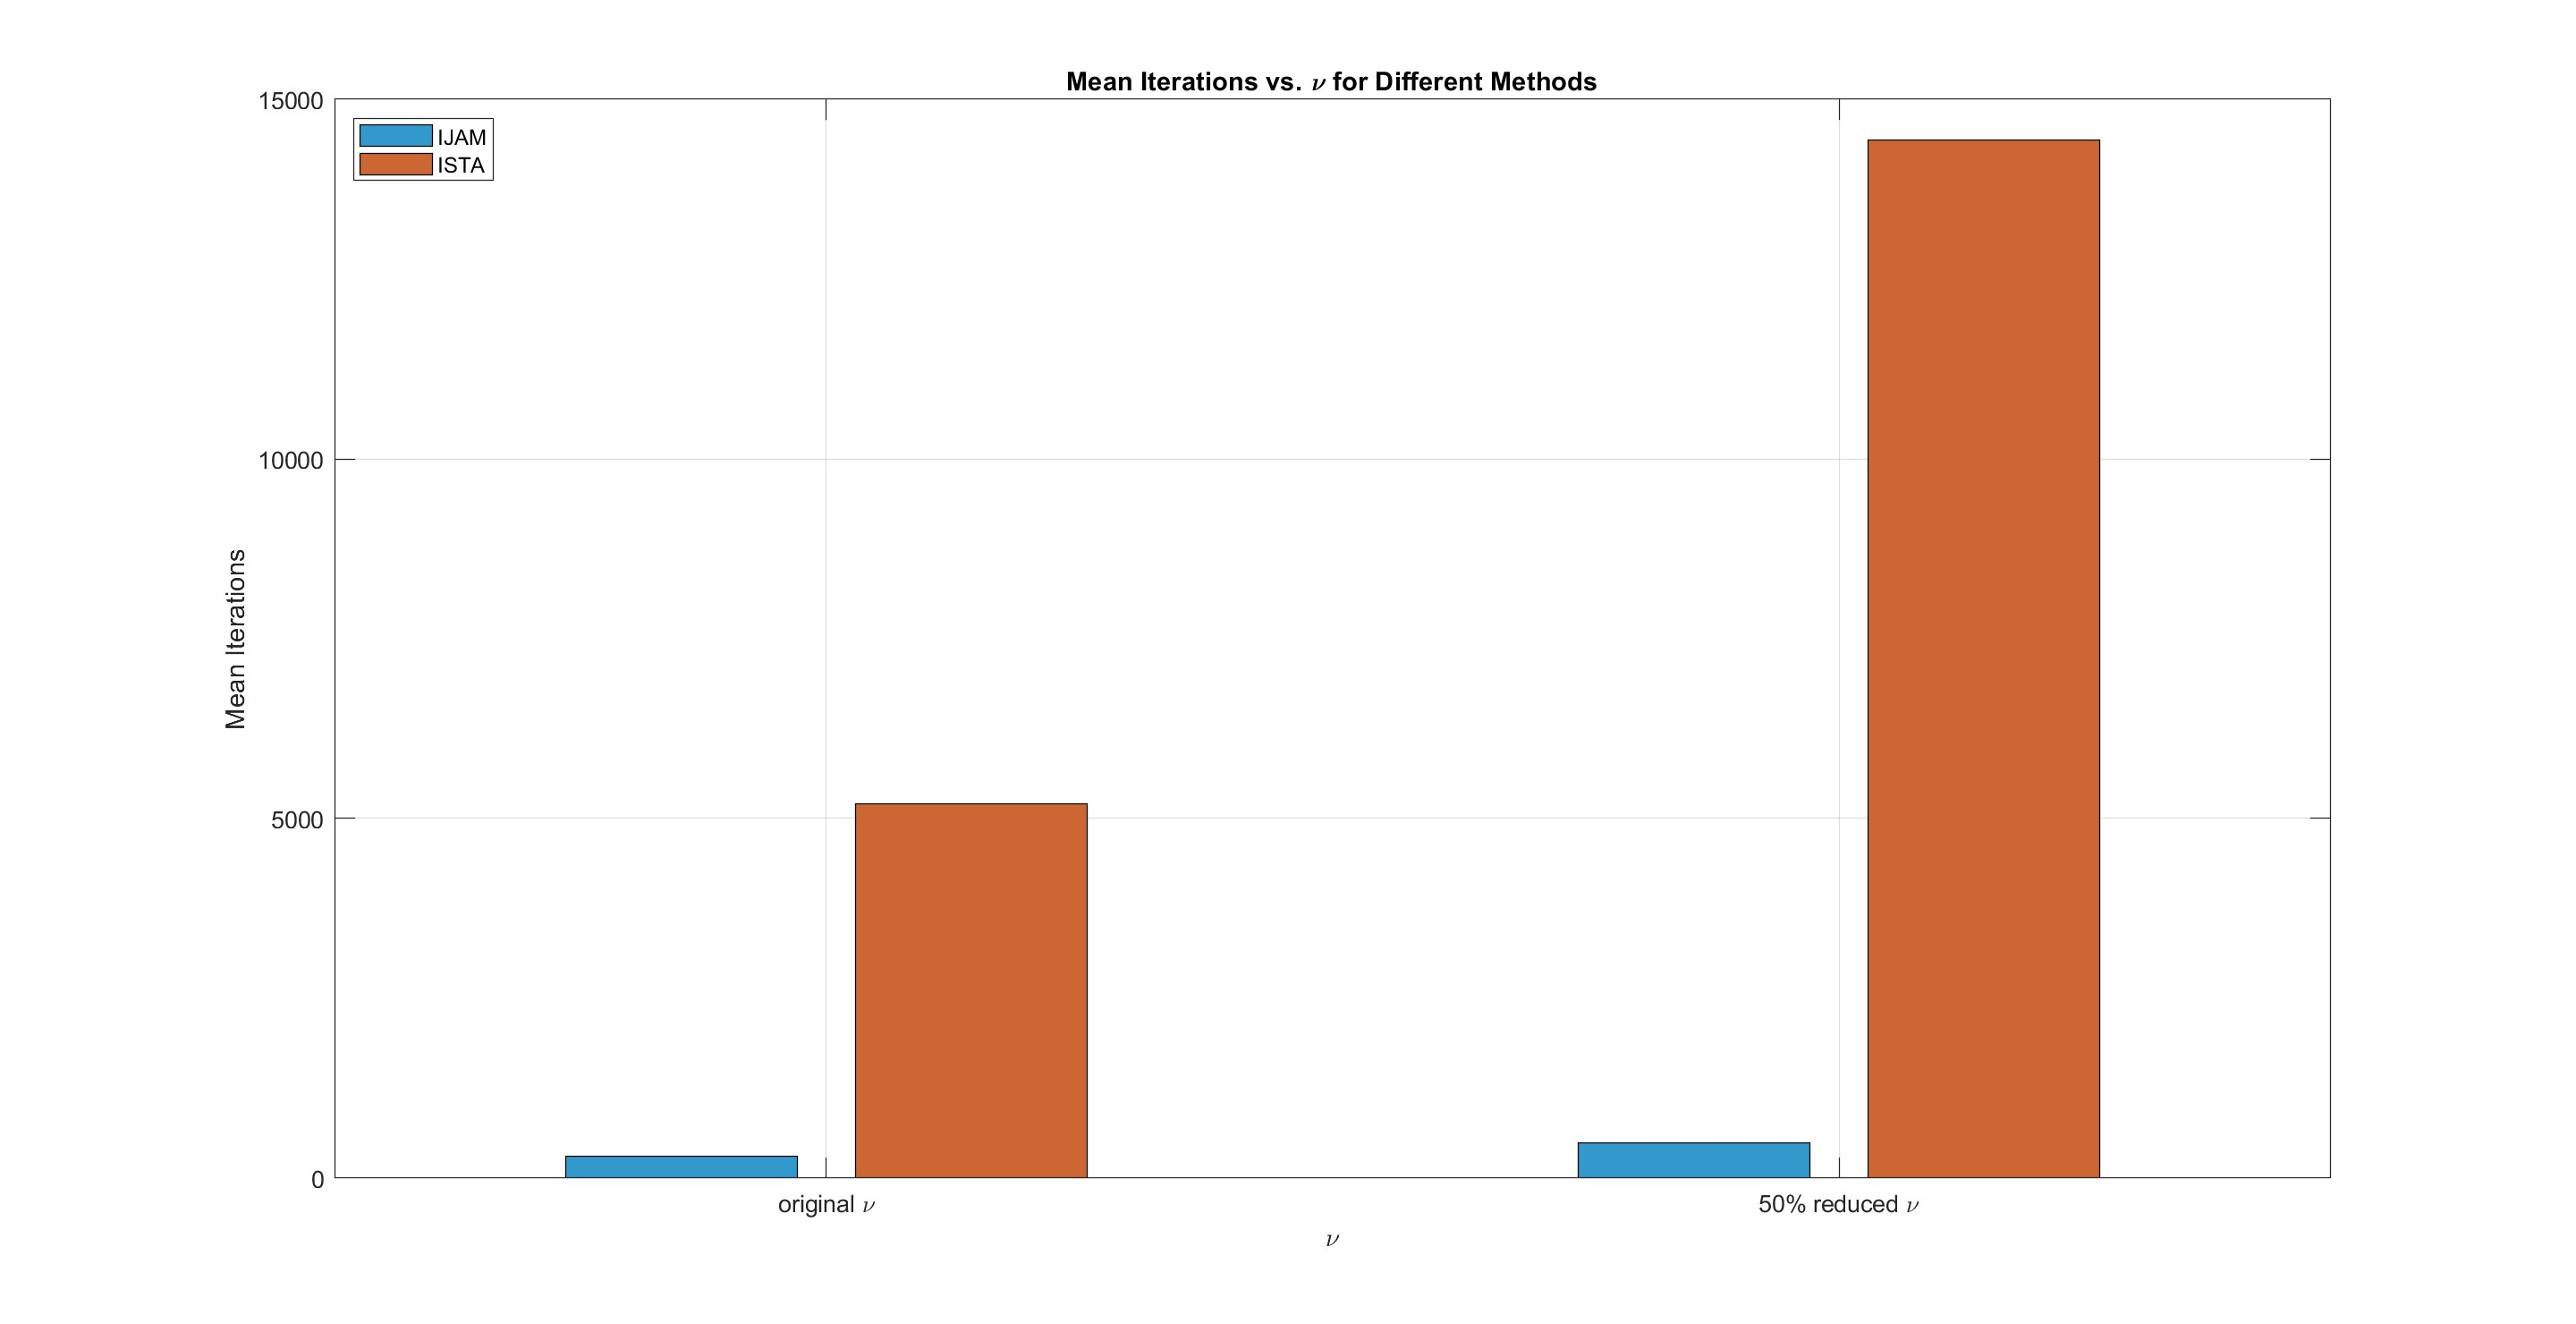
\includegraphics[width=0.65\textwidth]{iteration_vs_nu.jpg} % Adjust width as needed
    \caption{the plot of average number of iterations versus nu; the value of $\lambda$ is fixed to 1.}
    \label{fig:example}
\end{figure}

Having said that, for ISTA the value of the $\nu$ cannot be larger than a certain value; otherwise, the algorithm becomes numerically unstable. For ISTA, the Lipschitz condition ensures convergence by constraining 
\( \nu \) based on the spectral norm of \( C \):

\[
0 < \nu < \frac{2}{\|C\|^2}
\]

However, IJAM (Inertial Jacobi Alternating Minimization) is different because it does not use a direct gradient step for \( x \). Instead, it solves \( x \) via pseudo-inversion and applies an inertial term in the update for \( a \). This makes IJAM's convergence behavior less dependent on the Lipschitz constant and more on the inertia parameter \( \nu \) and the spectral properties of \( C \).

All in all, the optimal value of $\nu$ and $\lambda$ that guarantees a well performance cannot be introduced without a fixed $C$ matrix, which is the case while the algorithm were tested. Since ISTA and IJAM are used as the first step of ``my ISTA'' and ``my IJAM'', the same arguments holds for those two.

\subsubsection{Resilience to the number of the attacks}
Considering the dimension of the matrix $C$, the following necessary condition holds, intorducing the maximum possible number of the attacks that can be corrected:
\begin{equation}
h \leq \frac{q - n -1}{2}
\end{equation}
Considering the dimension of our problem:
\[
h \leq 7
\]

and there is proven another theory mentioning that $h$ errors are correctable if and only if:
\begin{equation}
\forall x \in \mathbb{R}^n, \ \|Cx\|_0 \geq 2h + 1
\end{equation}

However, not knowing $C$ this analize cannot be done, since we don't have any information about the dimension of the null space of $C$.

\begin{figure}[H] % h means "here", can also use t (top), b (bottom), p (page)
    \centering
    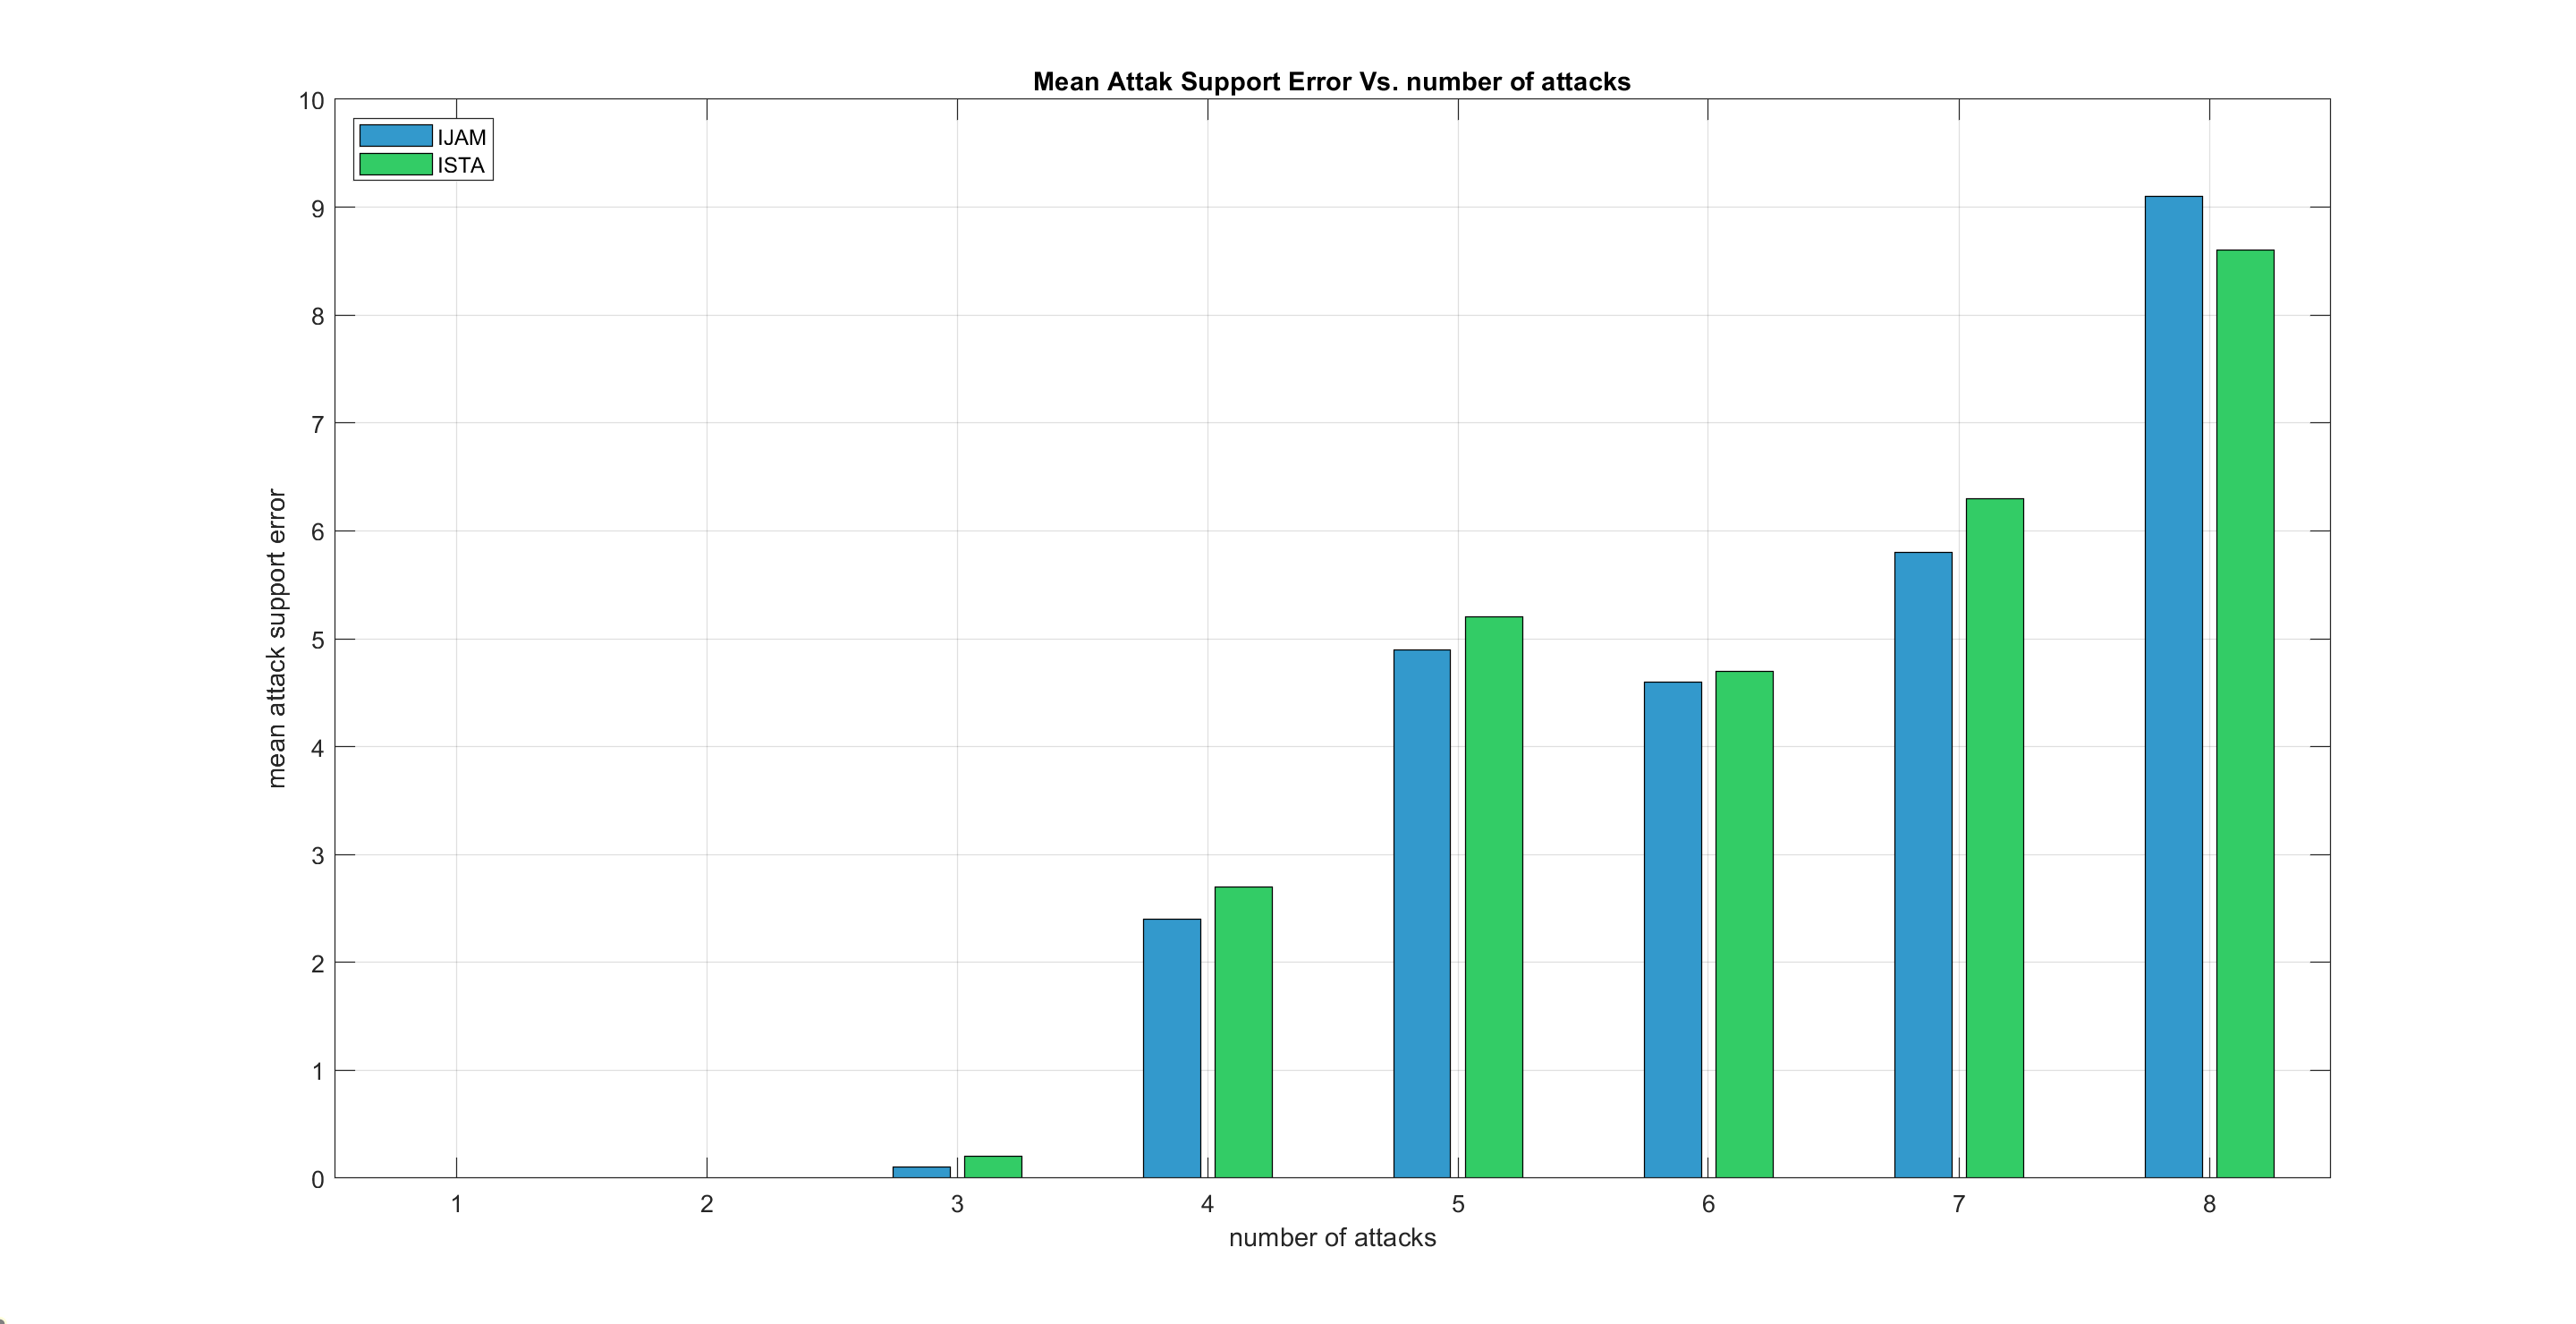
\includegraphics[width=0.75\textwidth]{resilience.png} % Adjust width as needed
    \caption{Mean attack support error in 20 run for different number of attacks.}
    \label{fig:example}
\end{figure}

It can be seen that by the time the number of attacks passes 7, almost all the time, the algorithm cannot detect the position of the attacks, supporting the theory regarding the number of correctable attack.
\section{Further Discussion}
\subsection{My Conjecture}
The position of the h-sparse attack can be found solely by solving the least-squares problem. Having solved the following least-squares problem:
\begin{equation}
    z = (C, I)^{+} y
\end{equation}
where
\begin{equation}
    z = 
    \begin{bmatrix}
        x \\
        a
    \end{bmatrix}
\end{equation}
a diagonal \( q \times q \) attack support matrix, \( M_a \), can be shaped which has 1 corresponding to the \( h \) components of \( a \), such that:
\begin{equation}
    z = G_{\text{sparse}}^{+} y
\end{equation}
where
 \begin{equation}
    G_{\text{sparse}} = 
    \begin{bmatrix}
        C M_a
    \end{bmatrix}
\end{equation} 

For $h = 1$, this method detect the correct position of the attack 80 percent of the time, without any iteration and just by two times solving a least-square problem! However, with $h = 2$ this number reduces to almost 50 percent of the time. In my opinion, this is more than a lucky guess and there must be a simple way using least square algorithm combined with some property of $C$ or some geometrical intrepretaiton, in order to find the position of the attacks.
\subsection{The energy of the attack}
If the energy of the attacks is considerable compared to the energy of the measurement vector Cx the aboved mentioned method can easily identify the attacks:
As an instance, the matrix \texttt{C = 0.01*randn(q,n)} is considered, while the value of the attack is kept constant. In this case, the attacks can be found up to a large number and with a good precision. The result can be seen in the following graphs.
\begin{figure}[H] % h means "here", can also use t (top), b (bottom), p (page)
    \centering
    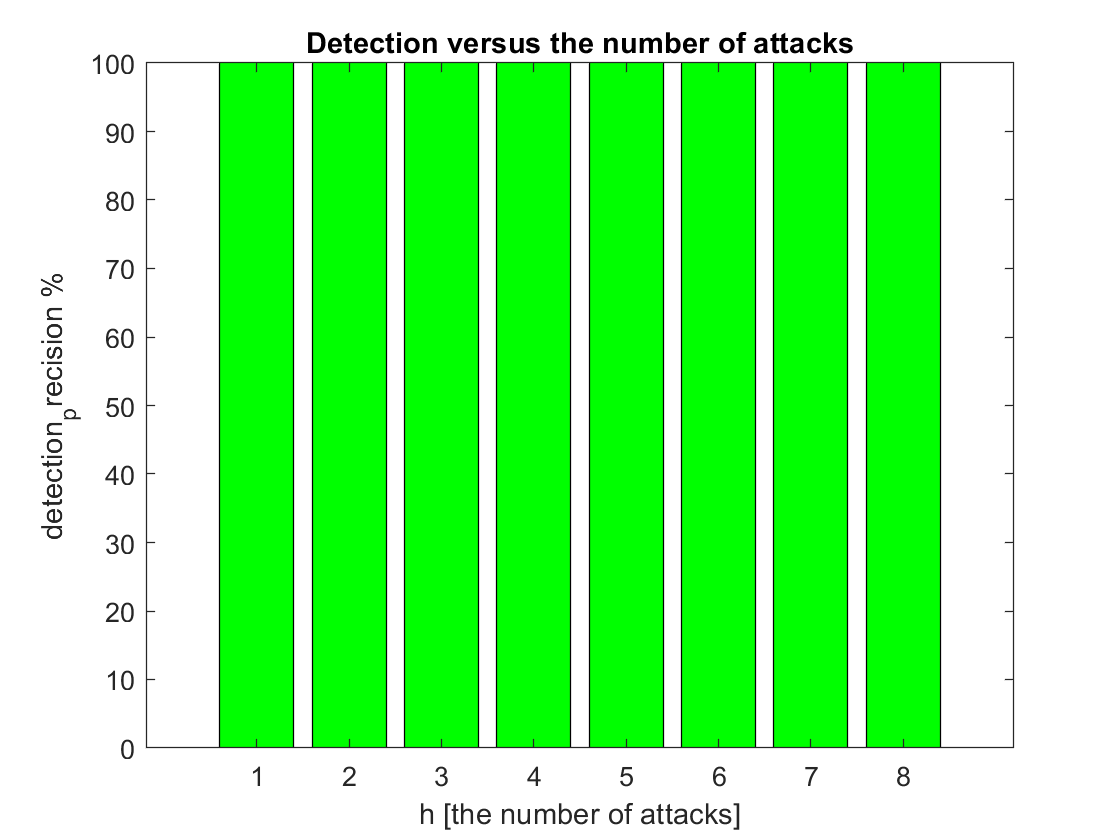
\includegraphics[width=0.65\textwidth]{detection_precision.png} % Adjust width as needed
    \caption{Detection versus the number of attacks}
    \label{fig:example}
\end{figure}

\begin{figure}[H] % h means "here", can also use t (top), b (bottom), p (page)
    \centering
    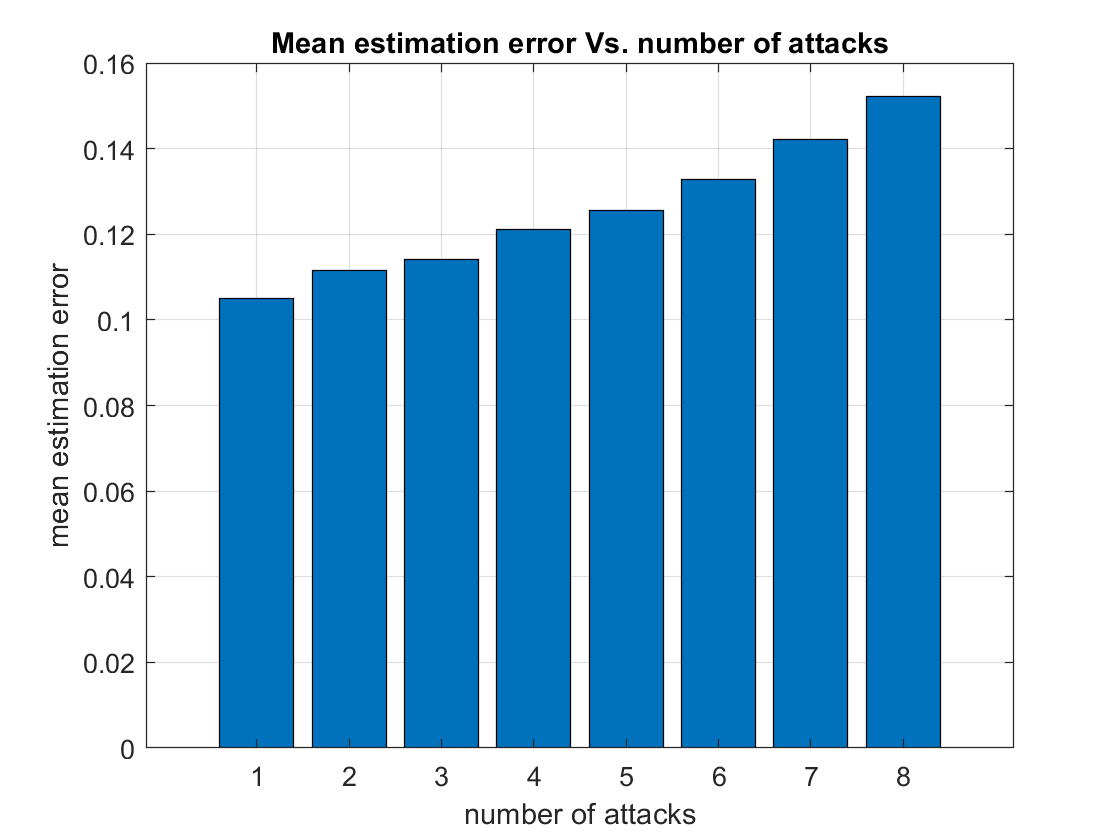
\includegraphics[width=0.65\textwidth]{mean_see.png} % Adjust width as needed
    \caption{Mean estimation error over; 1000 run for each number of attacks}
    \label{fig:example}
\end{figure}


\section{Conclusion}
It was observed that both IJAM and ISTA, are capable of detecting and correcting the effect of the attack by setting correctly the values of the hyper parameters. 

Regarding the precision of the algorithms, it was observed that my IJAM and my ISTA enjoy a higher precision compare to IJAM and ISTA, due to the fact that they almost reach the optimal solution of least-square algorithm. Nonetheless, still these two algorithms depend on IJAM and ISTA, in order to detect the position of the attacks.

 Regarding the hyperparameters, larger values of $\lambda$ leads to a faster convergence of the algorithm; however, in this case, the algorithms may overlook attacks with values smaller than $\lambda$. On the other hand, if $\lambda$ is selected too small, the algorithm considers noises and numerical inaccuracies as attack components. As to $\nu$, the numerical stability of the algorithms depends on this value, as it endows a sort of ``numerical inertia'' to the algorithms. Especially, ISTA is more dependent on this value as it uses gradient decent for converging to the estimation of the state vector, and for value of $\nu$ larger than Lipschitz condition, the algorithm becomes unstable. Stability of IJAM is less dependent on this value, but still the value of $\nu$ helps the stability of attack detection, since still a gradient decent is happening at each iteration for converging to the estimation of attack values.
 
Regarding relisience of the algorithms, considering the number of the states and the number of our sensors, thoretically, the algorithms cannot detect more than 7 number of attack. It was also observed that the attack support error grows as the number of attacks increases. In large scale systems, assuming that the number of attacks are small, these algorithms can be effective.
 
 











